\input ../SlidePreamble
\input ../preamble


\begin{document}

{\Huge

  \centerline{\bf TTIC 31230, Fundamentals of Deep Learning}
  \bigskip
  \centerline{David McAllester, Winter 2020}
  \vfill
  \vfil
  \centerline{Variational Autoencoders (VAEs)}
  \vfill
  \vfill

\slide{Latent Variable Models}

{\color{red} $$P_\Phi(y) = \sum_z\;P_\Phi(z)P_\Phi(y|z) = E_{z \sim P_\Phi(z)}\;P_\Phi(y|z)$$}

Or

\vfill
{\color{red} $$P_\Phi(y|x) = \sum_z\;P_\Phi(z|x)P_\Phi(y|z,x) = E_{z \sim P_\Phi(z|x)}\;P_\Phi(y|z,x)$$}

\vfill
Here {\color{red} $z$} is a latent variable.

\slide{Latent Variable Models}

{\color{red} $$P_\Phi(y) = \sum_z\;P_\Phi(z)P_\Phi(y|z) = E_{z \sim P_\Phi(z)}\;P_\Phi(y|z)$$}

Here we often think of $z$ as the causal source of $y$.

\vfill
For example $z$ might be a physical scene causing image $y$.

\vfill
Or $z$ might be the intended utterance causing speech signal $y$.

\vfill
In these situations a latent variable model should more accurately represents the distribution on $y$.

\slide{Latent Variable Models}

{\color{red} $$P_\Phi(y) = \sum_z\;P_\Phi(z)P_\Phi(y|z) = E_{z \sim P_\Phi(z)}\;P_\Phi(y|z)$$}

\vfill
$P_\Phi(z)$ is called the prior.

\vfill
Given an observation of $y$ (the evidence) $P_\Phi(z|y)$ is called the posterior.

\vfill
Variational Bayesian inference involves approximating the posterior.

\anaslide{Colorization with Latent Segmentation}
\medskip
\centerline{\includegraphics[width = 5in]{../images/colorizationGreg2}}
\centerline{$x$ \hspace{4em} $\hat{y}$ \hspace{4em} $y$}
\centerline{\huge Larsson et al., 2016}

\vfill
Colorization is a natural self-supervised learning problem --- we delete the color and then try to recover it from the grey-level image.

\vfill
Can colorization be used to learn segmentation?

\vfill
Segmentation is latent --- not determined by the color label.

\anaslide{Colorization with Latent Segmentation}
\medskip
\centerline{\includegraphics[width = 5in]{../images/colorizationGreg2}}
\centerline{$x$ \hspace{4em} $\hat{y}$ \hspace{4em} $y$}
\centerline{\huge Larsson et al., 2016}

\vfill
$x$ is a grey level image.

\vfill
$y$ is a color image drawn from $\pop(y|x)$.

\vfill
$\hat{y}$ is an arbitrary color image.

\vfill
$P_\Phi(\hat{y}|x)$ is the probability that model $\Phi$ assigns to the color image $\hat{y}$ given grey level image $x$.

\anaslide{Colorization with Latent Segmentation}
\medskip
\centerline{\includegraphics[width = 5in]{../images/colorizationGreg2}}
\centerline{$x$ \hspace{4em} $\hat{y}$ \hspace{4em} $y$}

\vfill
{\color{red} $$P_\Phi(\hat{y}|x) = \sum_z\;P_\Phi(z|x)P_\Phi(\hat{y}|z,x).$$}
\begin{eqnarray*}
\mbox{input}\; x \\
P_\Phi(z|x) & = & \ldots \;\;\mbox{\color{red} semantic segmentation} \\
P_\Phi(\hat{y}|z,x) & = & \ldots \;\;\mbox{\color{red} segment colorization} \\
\end{eqnarray*}

\anaslide{Assumptions}

\bigskip
\bigskip
We assume models $P_\Phi(z)$ and $P_\Phi(y|z)$ are both samplable and computable.

\vfill
In other words, we can sample from these distributions and for any given $z$ and $y$ we can compute $P_\Phi(z)$ and $P_\Phi(y|z)$.

\vfill
These are nontrivial assumptions.

\vfill
A loopy graphical model is neither (efficiently) samplable nor computable.

\slide{Cases Where the Assumptions Hold}

In CTC we have that $z$ is the sequence with blanks and $y$ is the result of removing the blanks from $z$.

\vfill
In a hidden markov model $z$ is the sequence of hidden states and $y$ is the sequence of emissions.

\vfill
An autoregressive model, such as an autoregressive language model, is both samplable and computable.

\slide{Image Generators}

\centerline{$z$\hspace{5in}$y_\Phi(z)$}
\centerline{\includegraphics[width=6in]{\images/generator2}}


\vfill
We can generate an image $y_\Phi(z)$ from noise $z$ where $p_\Phi(z)$ and $p_\Phi(y|z)$ are both samplable and computable.

\vfill
Typically $p_\Phi(z)$ is ${\cal N}(0,I)$ reshaped as $z[X,Y,J]$


\anaslide{Assumptions}

\bigskip
\bigskip
Even when $P_\Phi(z)$ and $P_\Phi(y|z)$ are samplable and computable we cannot typically compute $P_\Phi(y)$.

\vfill
Specifically, for $P_\Phi(y)$ defined by a GAN generator we cannot compute $P_\Phi(y)$ for a test image $y$.

\vfill
Hence it is not obvious how to optimize the fundamental equation.

$$\Phi^* = \argmin_\Phi\;E_{y \sim \pop}\;- \ln P_\Phi(y)$$

\slide{The Evidence Lower Bound (ELBO)}

{\huge
\begin{eqnarray*}
P_\Phi(y) & = & \frac{P_\Phi(y)P_\Phi(z|y)}{P_\Phi(z|y)} \\
\\
\\
& = & \frac{P_\Phi(z) P_\Phi(y|z)}{P_\Phi(z|y)} \\
\\
\\
\ln P_\Phi(y) & = & \ln \frac{P_\Phi(z) P_\Phi(y|z)}{P_\Phi(z|y)} \\
\\
\\
& = & E_{z \sim Q_\Phi(z|y)}\;\ln \frac{P_\Phi(z) P_\Phi(y|z)}{P_\Phi(z|y)}
\end{eqnarray*}
}

\slide{The Evidence Lower Bound (The ELBO)}

We introduce a samplable and computable model $Q_\Phi(z|y)$ to approximate $P_\Phi(z|y)$.

{\huge
\begin{eqnarray*}
 {\color{red} \ln P_\Phi(y)} & = & E_{z \sim Q_\Phi(z|y)} \ln \frac{P_\Phi(z)P_\Phi(y|z)}{P_\Phi(z|y)} \\
        \\
 & = & E_{z \sim Q_\Phi(z|y)} \left(\ln \frac{P_\Phi(z)P_\Phi(y|z)}{Q_\Phi(z|y)} + \ln \frac{Q_\Phi(z|y)}{P_\Phi(z|y)}\right) \\
 \\
  & = & \left(E_{z \sim Q_\Phi(z|y)} \ln \frac{P_\Phi(z)P_\Phi(y|z)}{Q_\Phi(z|y)}\right) + KL(Q_\Phi(z|y),P_\Phi(z|y)) \\
  \\
  & {\color{red} \geq} & {\color{red} E_{z \sim Q_\Phi(z|y)} \ln \frac{P_\Phi(z)P_\Phi(y|z)}{Q_\Phi(z|y)}}\;\;\mbox{The ELBO}
\end{eqnarray*}
}


\slide{The Variational Auto-Encoder (VAE)}

$$\Phi^* = \argmin_\Phi\; E_{y \sim \pop,\;z \sim Q_\Phi(z|y)}\;-\ln \frac{P_\Phi(z)P_\Phi(y|z)}{Q_\Phi(z|y)}$$

\slide{VAE generalizes EM}

Expectation Maximimization (EM) applies in the (highly special) case where the exact posterior $P_\Phi(z|y)$ is samplable and computable.
EM alternates exact optimization of $Q$ and $P$.

\vfill
VAE: $\Phi^* = \argmin_\Phi E_{y\sim \mathrm{Train},\;z \sim Q_\Phi(z|y)}\;\;- \ln \frac{P_\Phi(z,y)}{Q_\Phi(z|y)}$

\vfill
EM: $\Phi^{\color{red} t+1} =  \argmin_\Phi\;E_{y \sim \mathrm{Train}}\;E_{z \sim P_{\Phi^{\color{red} t}}(z|y)}\; - \ln P_\Phi(z,y)$ \\
\\
\centerline{\hspace{1em} Update \hspace{6em} Inference \hspace{2.5em}~}
\centerline{(M Step) \hspace{5em} (E Step) \hspace{1.5em}~}
\centerline{Hold $Q$ fixed \hspace{2.5em} $Q(z|y) = P_{\Phi^{\color{red} t}}(z|y)$ \hspace{0em}~}

\slide{Hard EM relies on Closed Form $Q^*$}

EM: $\Phi^{\color{red} t+1} =  \argmin_\Phi\;E_{y,z \sim P_{\Phi^{\color{red} t}}(z|y)}\; - \ln P_\Phi(z,y)$

\vfill
Hard EM: $\Phi^{\color{red} t+1} =  \argmin_\Phi\; E_{y, z = \argmax_z P_{\Phi^{\color{red} t}}(z|y)} \;- \ln P_\Phi(z,y)$

\vfill
This relies on $P_{\Phi^t}(z|y)$ being exactly computable so that the optimization over $Q$ in VAE has a closed form solution.

\vfill
For a ``hard VAE'' we need some way of training $Q$ other than sampling from it (see the slides on VQ-VAE).

\slide{The Reparameterization Trick}

\begin{eqnarray*}
- \ln P_\Phi(y) & \leq & E_{z \sim Q_\Phi(z|y)}\;-\ln \frac{P_\Phi(z)P_\Phi(y|z)}{Q_\Phi(z|y)} \\
\\
\\
& = & E_\epsilon\;-\ln \frac{P_\Phi(z)P_\Phi(y|z)}{Q_\Phi(z|y)}\;\;\;z := f_\Phi(y,\epsilon)
\end{eqnarray*}

\vfill
$\epsilon$ is parameter-independent noise.

\vfill
This supports SGD: $\nabla_\Phi \;E_{y,\epsilon}\; [\ldots] = E_{y,\epsilon}\; \nabla_\Phi\;[\ldots]$

\slide{Gaussian VAEs} 
$$\Phi^* = \argmin_\Phi E_{y,\epsilon}\;-\ln \frac{p_\Phi(z)p_\Phi(y|z)}{q_\Phi(z|y)}$$

{\color{red}
\begin{eqnarray*}
z & = & z_\Phi(y) + \sigma_\Phi(y) \odot \epsilon\;\;\;\epsilon \sim {\cal N}(0,I) \\
\\
q_\Phi(z[i]|y) & = & {\cal N}(z_\Phi(y)[i],\sigma_\Phi(y)[i]) \\
\\
p_\Phi(z[i]) & = & {\cal N}(\mu_p,\sigma_p[i]) \;\;\mbox{WLOG} = {\cal N}(0,1) \\
\\
p_\Phi(y|z) & = & {\cal N}(y_\Phi(z),\;\sigma^2I)
\end{eqnarray*}
}

\slide{$-\ln p_\Phi(y|z)$ as Distortion}

For $p_\Phi(y|z) \propto \exp(-||y - y_\Phi(z)||^2/(2\sigma^2))$ we get

\begin{eqnarray*}
\Phi^* & = & \argmin_{\Phi} E_{y,\epsilon}\;\;\;-\ln \frac{p_\Phi(z)}{q_\Phi(z|y)} - \ln p_\Phi(y|z) \\
\\
       & = & \argmin_{\Phi,\sigma} E_{y,\epsilon}\;\;\;-\ln \frac{p_\Phi(z)}{q_\Phi(z|y)} +\left(\frac{1}{2\sigma^2}\right)||y - y_\Phi(z)||^2 + d\ln \sigma
\end{eqnarray*}

\vfill
where

\centerline{$d$ is the dimension of $y$ and $\sigma^*  =  \sqrt{\frac{1}{d}\;E_{y,\epsilon}\; ||y - y_\Phi(z)||^2}$}

\slide{Posterior Collapse}

Assume Universal Expressiveness for $P_\Phi(y|z)$.

\vfill
This allows $P_\Phi(y|z) = \pop(y)$ independent of $z$.

\vfill
We then get a completely optimized model with $z$ taking a single (meaningless) determined value.

\vfill
$$Q_\Phi(z|y) = P_\Phi(z|y) = 1$$

\anaslide{Colorization with Latent Segmentation}
\medskip
\centerline{\includegraphics[width = 5in]{../images/colorizationGreg2}}
\centerline{$x$ \hspace{4em} $\hat{y}$ \hspace{4em} $y$}
\centerline{\huge Larsson et al., 2016}

\vfill
Can colorization be used to learn latent segmentation?

\vfill
We introduce a latent segmentation into the model.

\vfill
In practice the latent segmentation is likely to ``collapse'' because the colorization can be done just as well without it.


\slide{Independent Universality}

$$\Phi^* = \argmin_\Phi E_{y\sim \pop,\;z \sim Q_\Phi(z|y)}\;\;-\ln \frac{P_\Phi(z,y)}{Q_\Phi(z|y)}$$

\vfill
It is natural to assume  that $\Phi$ has independent parameters for each distribution.  In practice parameters are often shared.

\vfill
Since $\Phi$ can indepedently parameterize each distribution, we will often use an independent universality assumption
that $\Phi$ can represent any triple of distributions $Q(z|y)$, $P(z)$ and $P(y|z)$.


\slide{Independent Universality}

More formally, we will often assume that for any triple of distributions $Q(z|y)$, $P(z)$ and $P(y|z)$ there exists a $\Phi$ that {\color{red} simultaneously} satisfies

\begin{eqnarray*}
Q_\Phi(z|y) & = & Q(z|y) \\
P_\Phi(z) & = & P(z) \\
P_\Phi(y|z) & = & P(y|z)
\end{eqnarray*}

\vfill
This assumption allows each distribution to be independently optimized while holding the others fixed.

\slide{The $\beta$-VAE}

$\beta$-VAE: Learning Basic Visual Concepts With A
Constrained Variational Framework, Higgins et al., ICLR 2017.

\vfill
The $\beta$-VAE introduces a parameter $\beta$ allow control of the rate-distortion trade off.

\slide{Indeterminacy of the VAE}

VAE: $\Phi^* = \argmin_\Phi E_{y,\epsilon}\;-\ln \frac{P_\Phi(z)}{Q_\Phi(z|y)} - \ln P_\Phi(y|z)$

\vfill
Assuming independent universality we can optimize $P_\Phi(z)$ and $P_\Phi(y|z)$ while holding $Q_\Phi(z|y)$ fixed.
This gives

\begin{eqnarray*}
P^*(z) & = & = P_\popd(z) = E_y \;Q_\Phi(z|y) \\
\\
P^*(y|z) & = & P^*_\popd(y|z) \propto P(y,z) = \pop(y)Q_\Phi(z|y)
\end{eqnarray*}

\slide{Indeterminacy of the VAE}

\begin{eqnarray*}
\Phi^* & = & \argmin_\Phi E_{y,\epsilon}\;-\ln \frac{P_\popd(z)}{Q_\Phi(z|y)} - \ln P_\popd(y|z) \\
\\
& = & \argmin_\Phi \;\;\;I_\Phi(y,z)\; + \; H_\Phi(y|z) \\
\\
& = & \argmin_\Phi \;\;\;\;\; H_\popd(y)
\end{eqnarray*}

\vfill
But $H_\popd(y)$ is independent of $\Phi$.

\vfill
Any choice of $Q_\Phi(z|y)$ gives optimal modeling of $y$.

\slide{Indeterminacy of the VAE}

\begin{eqnarray*}
\Phi^* & = & \argmin_\Phi \; I_\Phi(y,z) + H_\Phi(y|z)
\end{eqnarray*}

\vfill
The choice of $Q_\Phi(z|y)$ does not influence the value of the objective function but controls $I(y,z)$.

\vfill
We have $0 \leq I(y,z) \leq H(y)$ with the full range possible.

\slide{The $\beta$-VAE}

To control $I(y,z)$ we introduce a weighting $\beta$

\begin{eqnarray*}
\Phi^* & = & \argmin_\Phi \; \beta I_\Phi(y,z) + H_\Phi(y|z) \\
\mbox{$\beta$-VAE}\;\; \Phi^* & = & \argmin_\Phi E_{y,\epsilon}\;-\beta \ln \frac{P_\Phi(z)}{Q_\Phi(z|y)} - \ln P_\Phi(y|z)
\end{eqnarray*}

\vfill
For $\beta < 1$ we no longer have an upper bound on $H_\popd(y)$ but we can force the use of $z$ (avoid posterior collapse).

\vfill
For $\beta > 1$ the bound on $H_\pop(y)$ becomes weaker and the latent variables carry less information.

\slide{RDAs vs. $\beta$-VAEs}

RDAs and $\beta$-VAEs are essentially the same.

\vfill
RDA: $\Phi^* = \argmin_\Phi E_{y,z \sim Q_\Phi(z|y)}\;-\ln \frac{P_\Phi(z)}{Q_\Phi(z|y)} + \lambda \mathrm{Dist}(y,y_\Phi(z))$

\vfill
$\beta$-VAE: $\Phi^* = \argmin_\Phi E_{y,z \sim Q_\Phi(z|y)}\;-\beta \ln \frac{P_\Phi(z)}{Q_\Phi(z|y)} \;-\;\ln P_\Phi(y|z)$

\slide{VAEs 2013}

\centerline{Sample {\color{red} $z \sim {\cal N}(0,I)$} and compute {\color{red} $y_\Phi(z)$}}

\vfill
\centerline{\includegraphics[width = 4in]{../images/VariationalFaces}}
\centerline{[Alec Radford]}

\slide{VAEs 2019}

\centerline{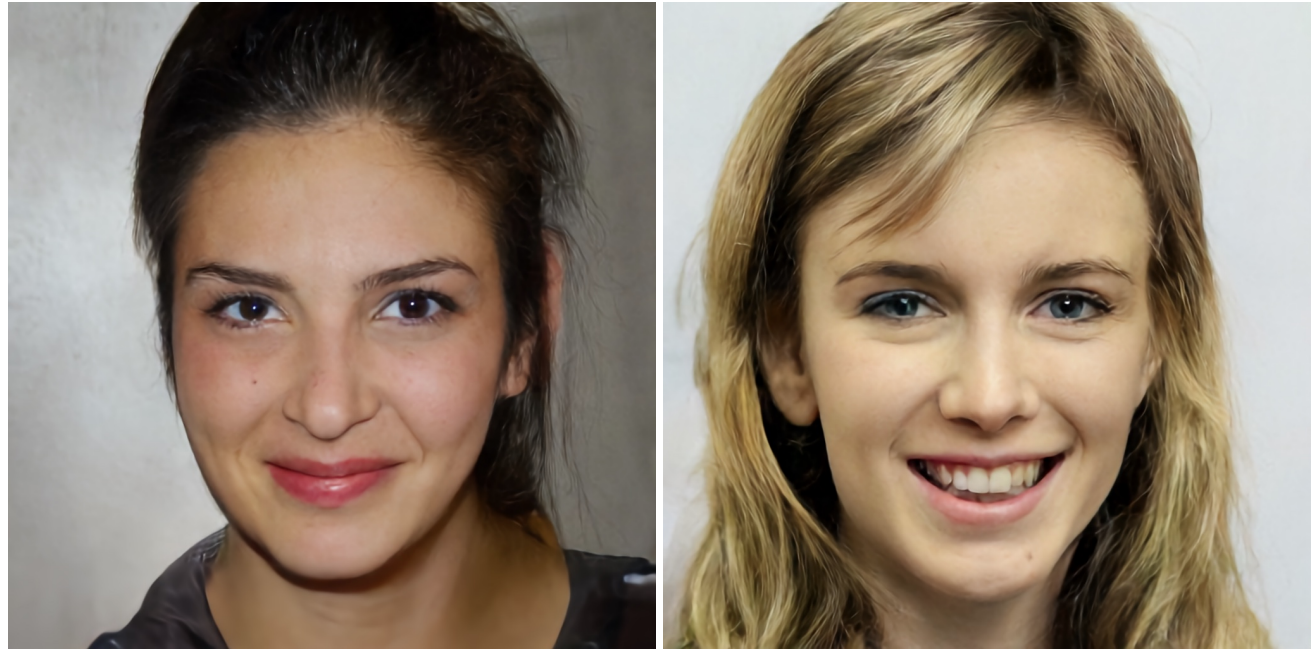
\includegraphics[width = 8in]{\images/VQ-VAE22}}

\vfill
VQ-VAE-2, Razavi et al. June, 2019

\slide{VAEs 2019}

\centerline{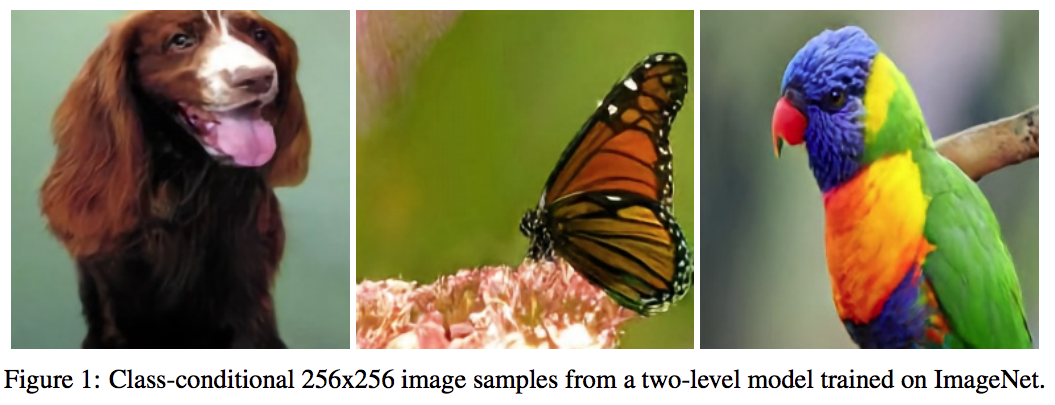
\includegraphics[width = 10in]{/users/davidmcallester/tex/images/VQ-VAE21}}

\vfill
VQ-VAE-2, Razavi et al. June, 2019


\slide{Vector Quantized VAEs (VQ-VAE)}

VQ-VAEs effectively perform $k$-means on vectors in the model so as to represent vectors by discrete cluster centers.

\vfill
For concreteness we will consider VQ-VAEs on images with a single layer of quantization.

\vfill
We use $x$ and $y$ for spatial image coordinates and use $s$ (for signal) to denote images.

\slide{VQ-VAE Encoder-Decoder}

We train a dictionary $C[K,I]$ where $C[k,I]$ is the center vector of cluster $k$.
\begin{eqnarray*}
L[X,Y,I] & = & \mathrm{Enc}_\Phi(s) \\
\\
z[x,y] & = & \argmin_k \;||L[x,y,I] - C[k,I]|| \\
\\
\hat{L}[x,y,I] & = & C[z[x,y],I] \\
\\
\hat{s} & = & \mathrm{Dec}_\Phi(\hat{L}[X,Y,I])
\end{eqnarray*}

\vfill
The ``symbolic image'' $z[X,Y]$ is the latent variable.

\slide{VQ-VAE as an RDA}

We will interpret the VQ-VAE as an RDA.

$$\Phi^*  =  \argmin_\Phi E_s\;I(s,z) + \lambda\mathrm{Dist}(s,\hat{s})$$

\vfill
The mutual information $I(s,z)$ is limited by the entropy of $z[X,Y]$ which can be no larger than $\ln K^{XY} = XY\ln K$.

\vfill
Maximizing $I(s,z)$ subject to this upper bound should reduce the distortion by providing the decoder with adequate information
about the image.

\slide{VQ-VAE Training Loss}

We preserve information about the image $s$ by minimizing the distortion between $L[X,Y,I]$ and its reconstruction $\hat{L}[X,Y,I]$.

\vfill
\begin{eqnarray*}
\Phi^* & = & \argmin_\Phi \;E_s\; \beta||L[X,Y,I] - \hat{L}[X,Y,I]||^2 + ||s -\hat{s}||^2
\end{eqnarray*}

\vfill
This is a two-level rate-distortion auto-encoder where the rate can be no larger than $XY\ln K$.

\slide{Parameter-Specific Learning Rates}

$$||L[X,Y,I] - \hat{L}[X,Y,I]||^2 = \sum_{x,y}\;||L[x,y,I] - C[z[x,y],I]||^2$$

\vfill
For the gradient of this they use

\begin{eqnarray*}
\mathrm{for}\;x,y\;\;L[x,y,I].\grad & \pluseq & 2\beta({L}[x,y,I]- C[z[x,y],I]) \\
\mathrm{for}\;x,y\;\;C[z[x,y],I].\grad & \pluseq & 2(C[z[x,y],I] - L[x,y,I])
\end{eqnarray*}

\vfill
This gives a parameter-specific learning rate for $C[K,I]$.

\vfill
Parameter-specific learning rates do not change the stationary points (the points where the gradients are zero).

\slide{The Relationship to $K$-means}

\begin{eqnarray*}
\mathrm{for}\;x,y\;\;C[z[x,y],I].\grad & \pluseq & 2(C[z[x,y],I] - L[x,y,I])
\end{eqnarray*}

\vfill
At a stationary point we get that $C[k,I]$ is the mean of the set of vectors $L[x,y,I]$ with $z[x,y] = k$ (as in $K$-means).

\slide{Straight Through Gradients}

The latent variables are discrete so some approximation to SGD must be used.

\vfill
They use ``straight-through'' gradients.

\begin{eqnarray*}
\mathrm{for}\;x,y\;\;L[x,y,I].\grad & \pluseq & \hat{L}[x,y,I].\grad
\end{eqnarray*}

\vfill
This assumes low distortion between $L[X,Y,I]$ and $\hat{L}[X,Y,I]$.

\slide{A Suggested Modification}

The parameter $\beta$ is paying two roles

\vfill
\begin{itemize}
\item It controls the relative weight of the two distortion losses.

\vfill
\item It controls the learning rate adjustment for the codebook.
\end{itemize}

\vfill
Shouldn't we have separate parameters for these two roles?

\slide{Training Phase II}

Once the model is trained we can sample images $s$ and compute the ``symbolic image'' $z[X,Y]$.

\vfill
Given samples of symbolic images $z[X,Y]$ we can learn an auto-regressive model of these symbolic images using a pixel-CNN.

\vfill
This yields a prior probability distribution $P_\Phi(z[X,Y])$ which provides a tighter upper bound on the rate.

\vfill
We can then measure compression and distortion for test images.  This is something GANs cannot do.

\slide{Multi-Layer Vector Quantized VAEs}
\centerline{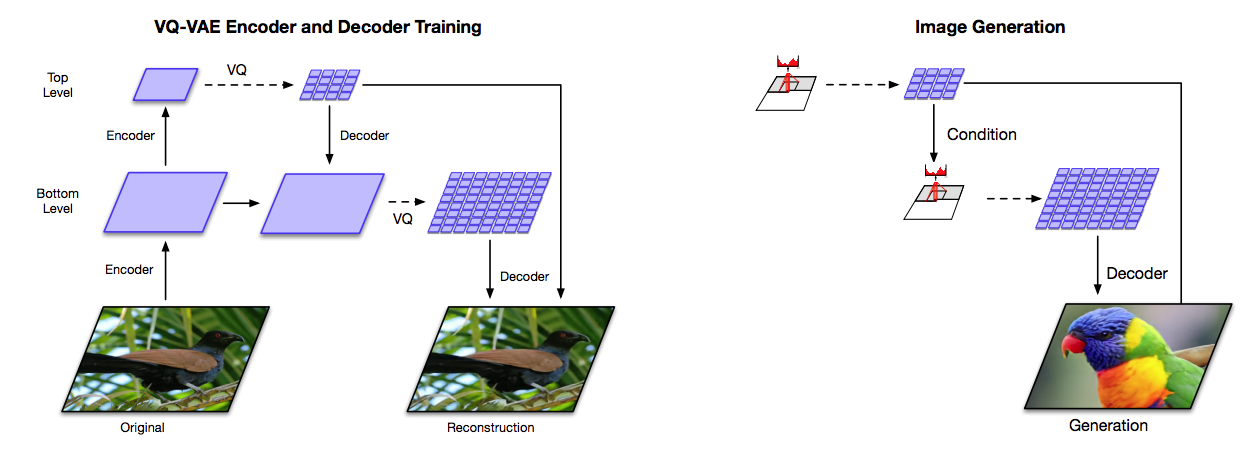
\includegraphics[width =10in]{\images/VQ-VAE24}}

\slide{Quantitative Evaluation}

The VQ-VAE2 paper reports a classification accuracy score (CAS) for class-conditional image generation.

\vfill
We generate image-class pairs from the generative model trained on the ImageNet training data.

\vfill
We then train an image classifier from the generated pairs and measure its accuracy on the ImageNet test set.

\vfill
\centerline{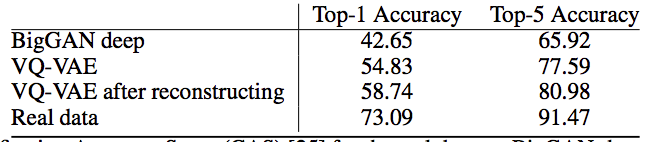
\includegraphics[width=7in]{\images/VQ-VAE23}}

\slide{Direct Rate-Distortion Evaluation.}

Rate-distortion metrics for image compression to discrete representations support unambiguous rate-distortion evaluation.

\vfill
Rate-distortion metrics also allow one to explore the rate-distortion trade-off.

\vfill
\centerline{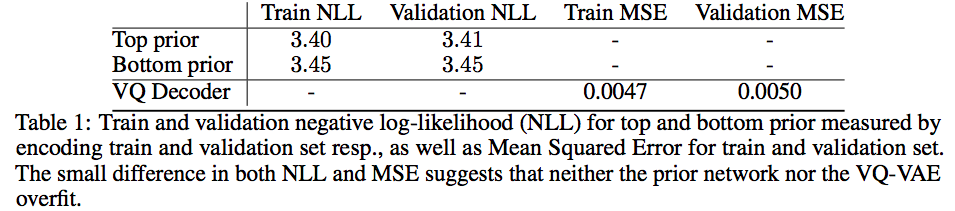
\includegraphics[width = 10in]{\images/VQVAE2Scores}}

\slide{Image Compression}

\vfill
\centerline{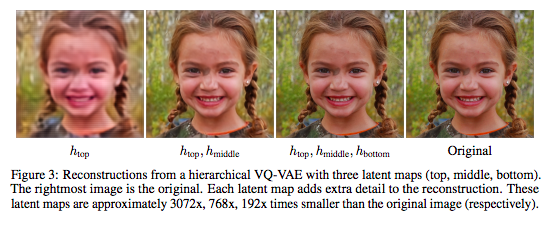
\includegraphics[width = 10in]{\images/VQgirl}}


\slide{Vector Quantization (Emergent Symbols)}

Vector quantization represents a distribution (or density) on vectors with a discrete set of embedded symbols.

\vfill
Vector quantization optimizes a rate-distortion tradeoff for vector compression.

\vfill
The VQ-VAE uses vector quantization to construct a discrete representation of images and hence a measurable image compression rate-distortion trade-off.

\slide{Symbols: A Better Learning Bias}

Do the objects of reality fall into categories?

\vfill
If so, shouldn't a learning architecture be designed to categorize?

\vfill
Whole image symbols would yield emergent whole image classification.

\slide{Symbols: Improved Interpretability}

Vector quantization shifts interpretation from linear threshold units to the emergent symbols.

\vfill
This seems related to the use of t-SNE as a tool in interpretation.


\slide{Symbols: Unifying Vision and Language}

Modern language models use word vectors.

\vfill
Word vectors are embedded symbols.

\vfill
Vector quantization also results in models based on embedded symbols.

\slide{Symbols: Addressing the ``Forgetting'' Problem}
When we learn to ski we do not forget how to ride a bicycle.

\vfill
However, when a model is trained on a first task, retraining on a second tasks degrades performance on the first (the model ``forgets'').

\vfill
But embedded symbols can be task specific.

\vfill
The embedding of a task-specific symbol will not change when training on a different task.


\slide{Symbols: Improved Transfer Learning.}

Embedded symbols can be domain specific.

\vfill
Separating domain-general parameters from domain-specific parameters may improve transfer between domains.

\slide{Unsupervised Machine Translation}

We can treat the German sentence $z$ as a latent variable in a probability model of a English sentence $y$.

$$\Phi^* = \argmin_\Phi\;E_{y,z \sim Q_\Phi(z|y)} \; \;-\beta \ln \frac{P_\Phi(z)}{Q_\Phi(z|y)} - \ln P_\Phi(y|z)$$

\vfill
Here $P_\Phi(z)$ can be a trained language model for German and $P_\Phi(y|z)$ and $Q_\Phi(z|y)$ are translation models.

\slide{Unsupervised Machine Translation}

In practice we use ``backtranslation''

$$\Phi^* = \argmin_\Phi\;\begin{array}{ll} & E_{y\sim \pop_y,\;z \sim Q_\Phi(z|y)} \; \;-\ln P_\Phi(y|z) \\ \\
+ & E_{z \sim \pop_z,\;y \sim P_\Phi(y|z)} \; \;-\ln Q_\Phi(z|y) \end{array}$$

\slide{END}

\end{document}
